\documentclass[10pt]{article}
\usepackage{amsmath} 
\usepackage{fontspec}
\setmainfont{JetBrainsMono NFM}
\setmainfont[NFSSFamily=dayrom]{JetBrains Mono}
\usepackage[a4paper, margin=12mm]{geometry}
\usepackage{graphicx}
\graphicspath{ {./images/} }

\usepackage{amsmath}

\DeclareSymbolFont{digits}{TU}{dayrom}{m}{n}
\AtBeginDocument{
	\DeclareMathSymbol{0}{\mathalpha}{digits}{`0}
	\DeclareMathSymbol{1}{\mathalpha}{digits}{`1}
	\DeclareMathSymbol{2}{\mathalpha}{digits}{`2}
	\DeclareMathSymbol{3}{\mathalpha}{digits}{`3}
	\DeclareMathSymbol{4}{\mathalpha}{digits}{`4}
	\DeclareMathSymbol{5}{\mathalpha}{digits}{`5}
	\DeclareMathSymbol{6}{\mathalpha}{digits}{`6}
	\DeclareMathSymbol{7}{\mathalpha}{digits}{`7}
	\DeclareMathSymbol{8}{\mathalpha}{digits}{`8}
	\DeclareMathSymbol{9}{\mathalpha}{digits}{`9}
}

% Footer-Einstellungen
\usepackage{fancyhdr}
\usepackage{amsmath}
\usepackage{datetime}
\newdateformat{mydate}{\twodigit{\THEDAY}.\twodigit{\THEMONTH}.\THEYEAR}
\mydate
\pagestyle{fancy}
\fancyhf{} % Löscht alle Kopf- und Fusszeilen
\fancyfoot[C]{\thepage\ -\ \today\ \copyright\ Bastian\ Kind,\ James\ Binks,\ Mark\ Matkovic\ und\ David\ Hafner} % Setzt den Footer

\title{DFB Entdecker App}
\author{Bastian Kind, James Binks, Mark Matkovic und David Hafner}

\begin{document}
	\maketitle
	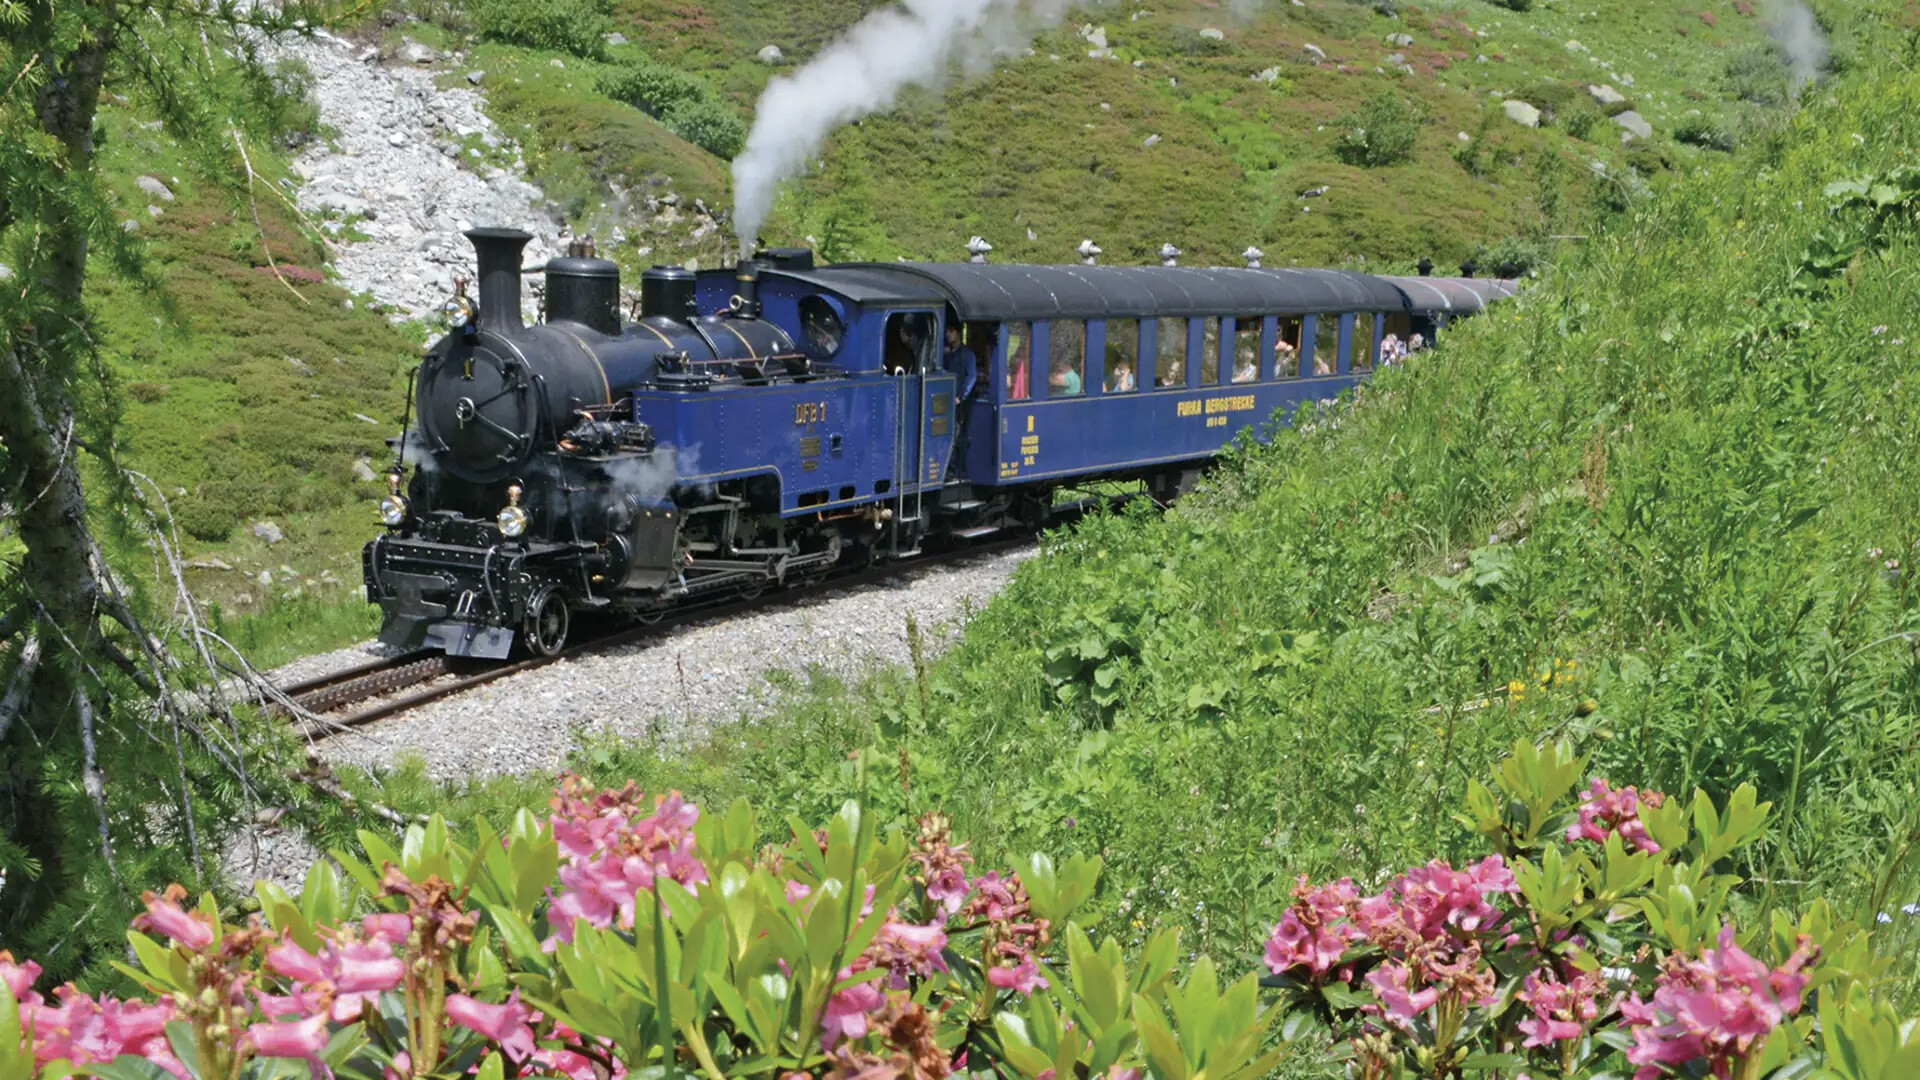
\includegraphics[width=17.5cm]{title}
	\pagebreak
	\tableofcontents
	\pagebreak
	\section{Band A}
	\subsection{Anforderungsanalyse}
	\subsubsection[Wer]{Wer benutzt die App?}
	\begin{itemize}
		\item Familien mit Kindern (z. B. als Freizeit-Ausflug)
		\item Rentner / ältere Menschen (Interesse an Geschichte und Eisenbahn)
		\item Erwachsene allgemein (z. B. Eisenbahnbegeisterte, Touristen)
		\item Schulklassen (für interaktive, spielerische Lernmöglichkeiten)
	\end{itemize}
	\subsubsection[Wo]{Wo wird die App verwendet?}
	\begin{itemize}
		\item Entlang der Furka-Bergstrecke, einer historischen Dampfbahnstrecke
		\item Draussen (z. B. auf Bahnhöfen, an Brücken, bei Aussichtspunkten)
		\item Oft ohne Mobilfunknetz -> App muss offlinefähig sein
		\item Unterwegs mit dem Zug oder zu Fuss an Haltepunkten
	\end{itemize}
	\subsubsection[Was]{Was muss die App können?}
	\begin{itemize}
		\item QR-Codes an Infopunkten scannen -> Inhalte anzeigen (Text, Bilder, Videos, Audio)
		\item Karte mit GPS nutzen -> aktuelle Position und nahegelegene Punkte anzeigen
		\item Quiz- oder Rätsel-Funktion -> spielerisches Lernen
		\item Tagebuch- oder Sammelfunktion („Meine liebsten Sehenswürdigkeiten“)
		\item Inhalte in mehreren Sprachen (D/E/F/I), evtl. auch einfache Sprache
		\item Inhalte offline verfügbar
		\item Datenschutzkonform -> keine Registrierung, keine Standortüberwachung
	\end{itemize}
	\subsubsection[Womit]{Technische Rahmenbedingungen}
	\begin{itemize}
		\item Smartphone oder Tablet, Android und iOS
		\item Ressourcenschonendes Design (damit es auch auf älteren Geräten läuft)
		\item App soll Inhalte aus CMS (z. B. Texte, Medien) beziehen
		\item Kein Internet nötig unterwegs (alle Inhalte offline verfügbar)
		\item Barrierefreiheit: Vorlesefunktion, grosse Schrift, starke Kontraste
	\end{itemize}
	\subsection{Vorgehensmodell}
	\subsection{Nutzungskontext}
	\subsection{Benutzereigenschaften}
	\subsection{Nutzungsanforderungen}
\end{document}